\documentclass[a4paper]{article}
\usepackage{a4wide}
\usepackage{amsmath}
\usepackage{amsfonts}
  \DeclareMathOperator*{\argmax}{arg\,max}
  \newcommand{\ex}[1]{{\mathbb E}\left[ #1 \right]}
  \newcommand\norm[1]{\left\lVert#1\right\rVert}
\usepackage{booktabs}
\usepackage{csquotes}
\usepackage{upquote}
\usepackage{float}
\usepackage{graphicx}
\usepackage{enumerate}
\usepackage{subcaption}
\usepackage[most]{tcolorbox}
\usepackage{xcolor}
\usepackage{varwidth} 


\title{Pattern and Speech Recognition WS2015-16 \\ Exercise 8}
\author{Atanas Poibrenski(2554135), Marimuthu Kalimuthu(2557695), Furkat Kochkarov(2557017)}

\begin{document}
	\tcbset{
		enhanced,
		colback=red!5!white,
		boxrule=0.1pt,
		colframe=red!75!black,
		fonttitle=\bfseries
	}

\maketitle 
\begin{center}
	\textbf{Decision Trees}
\end{center}

\section*{1 Loading the data}
\begin{enumerate}
	\item[ \textbf{Ex.1} ] Done.
	\item[ \textbf{Ex.2} ] See ``data\_preparation.m"
	\begin{figure}[H]
		\begin{center}
			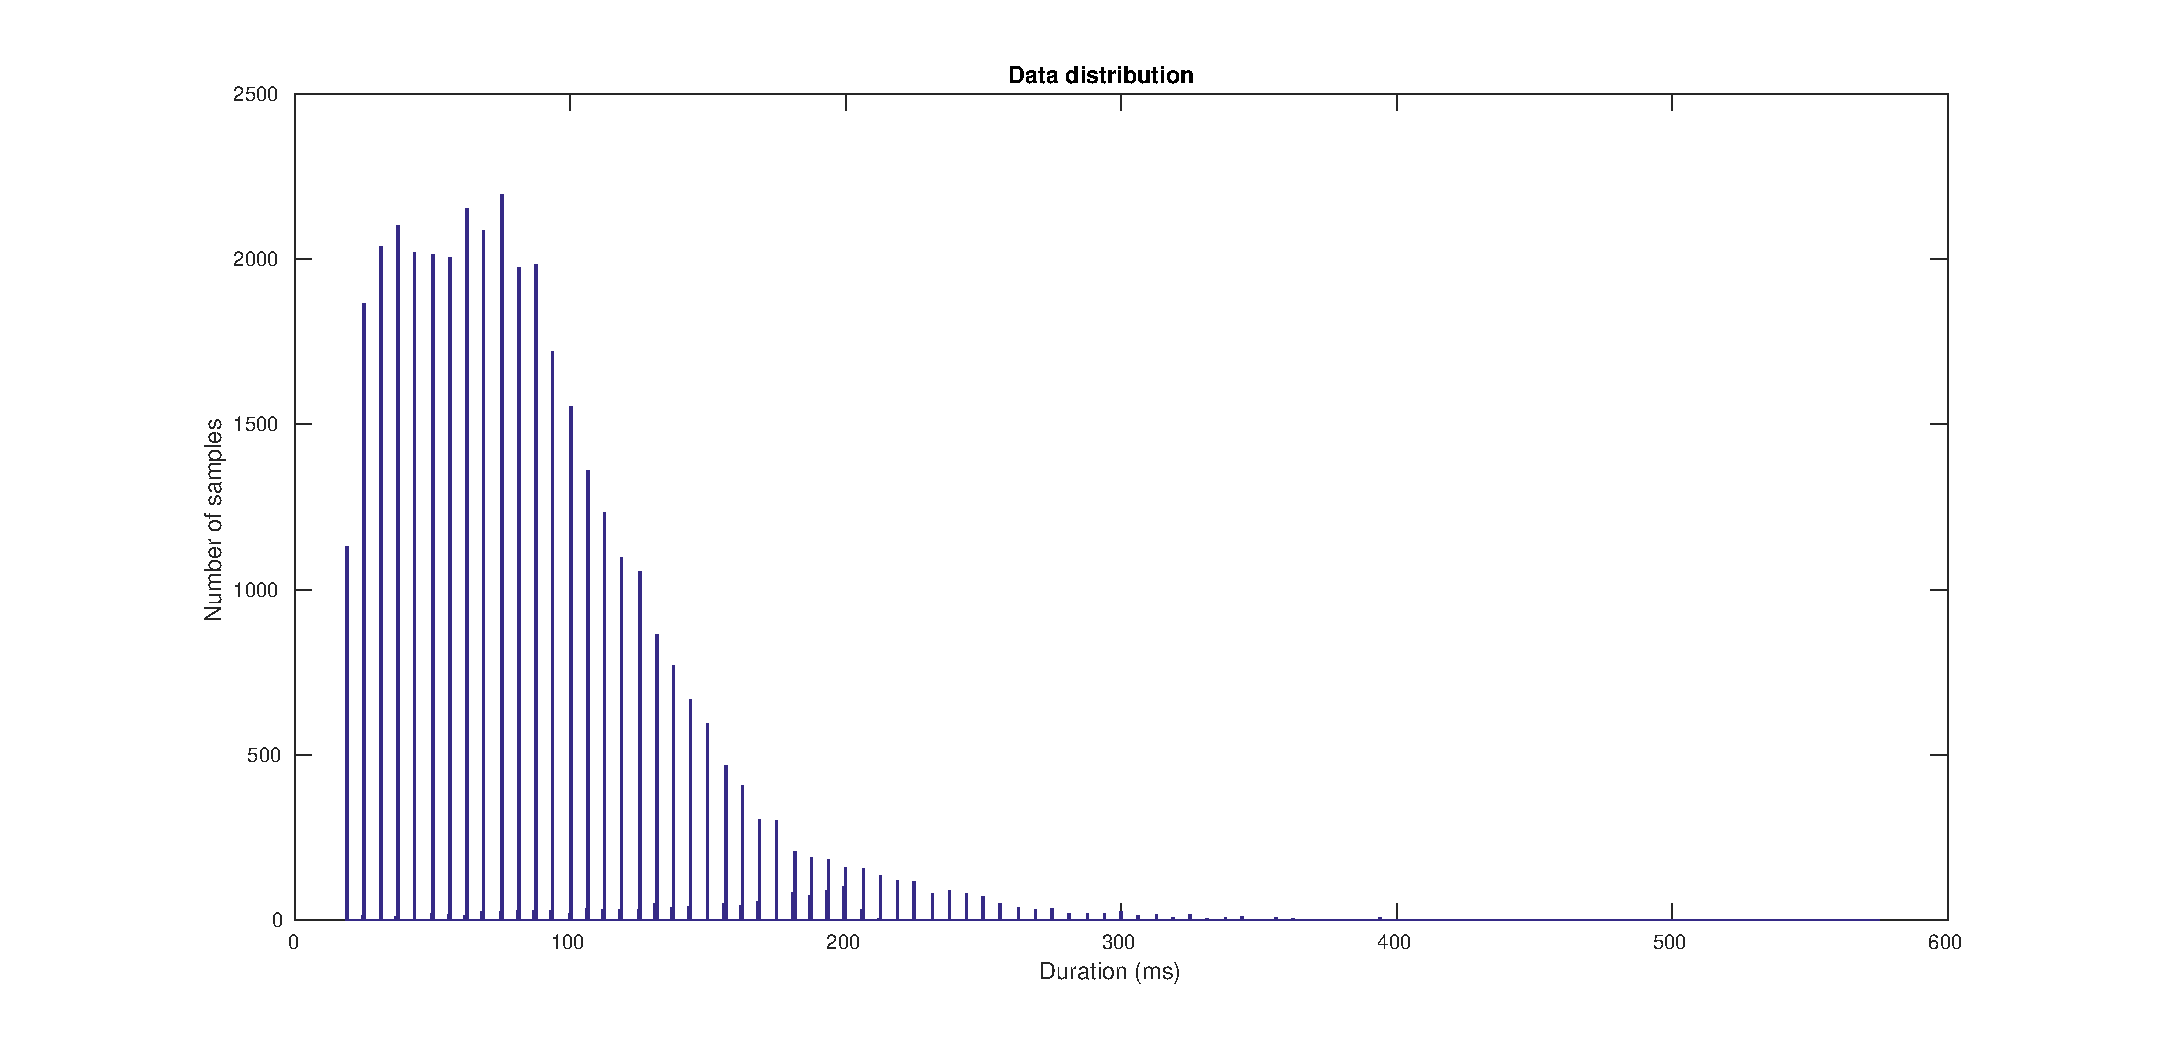
\includegraphics[width=1.1\textwidth]{plot.eps}
			\caption{Histogram plot of phoneme durations}\label{fig:hist}
		\end{center}
	\end{figure}

	\item[ \textbf{Ex.3} ] \textbf{Bonus}: \newline
	Yes, we can use Gaussian Mixture Models for duration modeling. We create 60 components which is the total number of phoneme types(i.e., Vowel, Consonant) and fit a Gaussian to each. Then a new phoneme comes we predict the cluster with highest probability which contains the phoneme.
	
	\item[ \textbf{Ex.4} ] \textbf{Bonus}: \newline
	In GMM, we always have a certain probability of a phoneme belonging to particular cluster. In decision trees, a phoneme either belongs to certain type or not.(i.e. it is a binary decision).

	\item[ \textbf{Ex.5} ] Divide dataset: \newline
	We use matlab's `dividerand' function which gives random indices. (i.e. shuffle the data). Then we get the following counts: \newline
	\begin{tcolorbox}
       Training set (90\%) -- 34980 samples \newline
	   Validation set (5\%) -- 1943 samples \newline
	   Test set (5\%) -- 1943 samples
	\end{tcolorbox}
\end{enumerate}

\section*{2 Decision Tree clustering}
\subsection*{2.1 Preliminary work}

\begin{enumerate}
	\item[ \textbf{Ex.6} ] data structure: \newline
	We use matlab `struct' which has three attributes `value', `left', and `right'.
	Since we will be using recursion for creation of the tree, it is convenient to use it.
\end{enumerate}

\subsection*{2.2 Criterion}
\begin{enumerate}
	\item[ \textbf{Ex.7} ] find\_question: \newline
	   See `find\_question.m'. We calculate the entropy impurity for each question and choose the one with minimum impurity.
	   
	\item[ \textbf{Ex.8} ] eval\_tree: \newline
	 See `eval\_tree.m'. It is calling `classify\_by\_tree' for each data point in the given corpus. And it is calculating the RMSE.

\end{enumerate}


\subsection*{2.3 Training the tree}
\begin{enumerate}
	\item[ \textbf{Ex.9} ]	`train\_tree'
	See `train\_tree.m'. It is creating the tree in a recursive manner with a fixed depth for the tree. \newline
	In `training.m', we call `train\_tree.m' in an iterative deepening manner. This way we get trees with different depths, so that we can apply the stopping criteria where we evaluate two trees of different depths.
	
\end{enumerate}


\section*{3 Some analysis}
	\begin{enumerate}
		\item[ \textbf{Ex.10} ]
		  The same as we did in Ex.5 will work here too.
		  
		\item[ \textbf{Ex.11} ] Our training of the tree is not working as desired.
		
	    \item[ \textbf{Ex.12} ] Our training of the tree is not working as desired.
	    
	\end{enumerate}

\end{document}
